\documentclass[10pt,a4paper,twocolumn]{article}
\usepackage[top=1.2cm,bottom=1.25cm,left=1.35cm,right=1.35cm]{geometry}
\usepackage{graphicx,booktabs,microtype,xcolor,amsmath,array,tabularx}
\usepackage[font=small,labelfont=bf,skip=2.5pt]{caption}
\usepackage[font=footnotesize]{subcaption}
\usepackage{titlesec}
\usepackage[T1]{fontenc}
\usepackage{lmodern}
\usepackage[colorlinks=true,linkcolor=NavyB,citecolor=NavyB,urlcolor=NavyB]{hyperref}

\definecolor{NavyB}{RGB}{20,60,120}

\titleformat{\section}{\normalfont\sffamily\bfseries\normalsize\color{NavyB}}{\thesection}{0.55em}{}
\titleformat{\subsection}{\normalfont\sffamily\bfseries\small\color{NavyB!85!black}}{\thesubsection}{0.45em}{}
\titlespacing{\section}{0pt}{6pt plus 1pt minus 1pt}{2pt}
\titlespacing{\subsection}{0pt}{4.5pt plus 1pt minus 1pt}{1pt}
\setlength{\columnsep}{0.65cm}
\setlength{\abovedisplayskip}{4pt}\setlength{\belowdisplayskip}{4pt}
\setlength{\textfloatsep}{7pt plus 2pt minus 2pt}
\setlength{\floatsep}{7pt plus 2pt minus 2pt}
\setlength{\intextsep}{7pt plus 2pt minus 2pt}
\renewcommand{\arraystretch}{1.05}
\newcommand{\tw}[1]{\texttt{\footnotesize #1}}
\newcommand{\thm}[1]{{\footnotesize\textsf{#1}}}
\renewcommand{\topfraction}{0.9}\renewcommand{\dbltopfraction}{0.9}
\renewcommand{\textfraction}{0.07}\renewcommand{\floatpagefraction}{0.8}
\renewcommand{\dblfloatpagefraction}{0.8}
\pagestyle{plain}

\begin{document}

\twocolumn[{%
\begin{center}
{\sffamily\bfseries\LARGE\color{NavyB} Theme Worlds\par}
\vspace{1pt}
{\sffamily\large Seamless Wrap-Around Panoramas from Stable Diffusion v1.5,
via a From-Scratch MultiDiffusion Sampler\par}
\vspace{4pt}
{\sffamily\small \textbf{Marlen Melis}\;\;$\cdot$\;\;
KAIST AIC.20000 \emph{Introduction to AI Computing} (Fall 2026)\;\;$\cdot$\;\;Mini-Project Write-Up\par}
\vspace{5pt}
\end{center}
\centering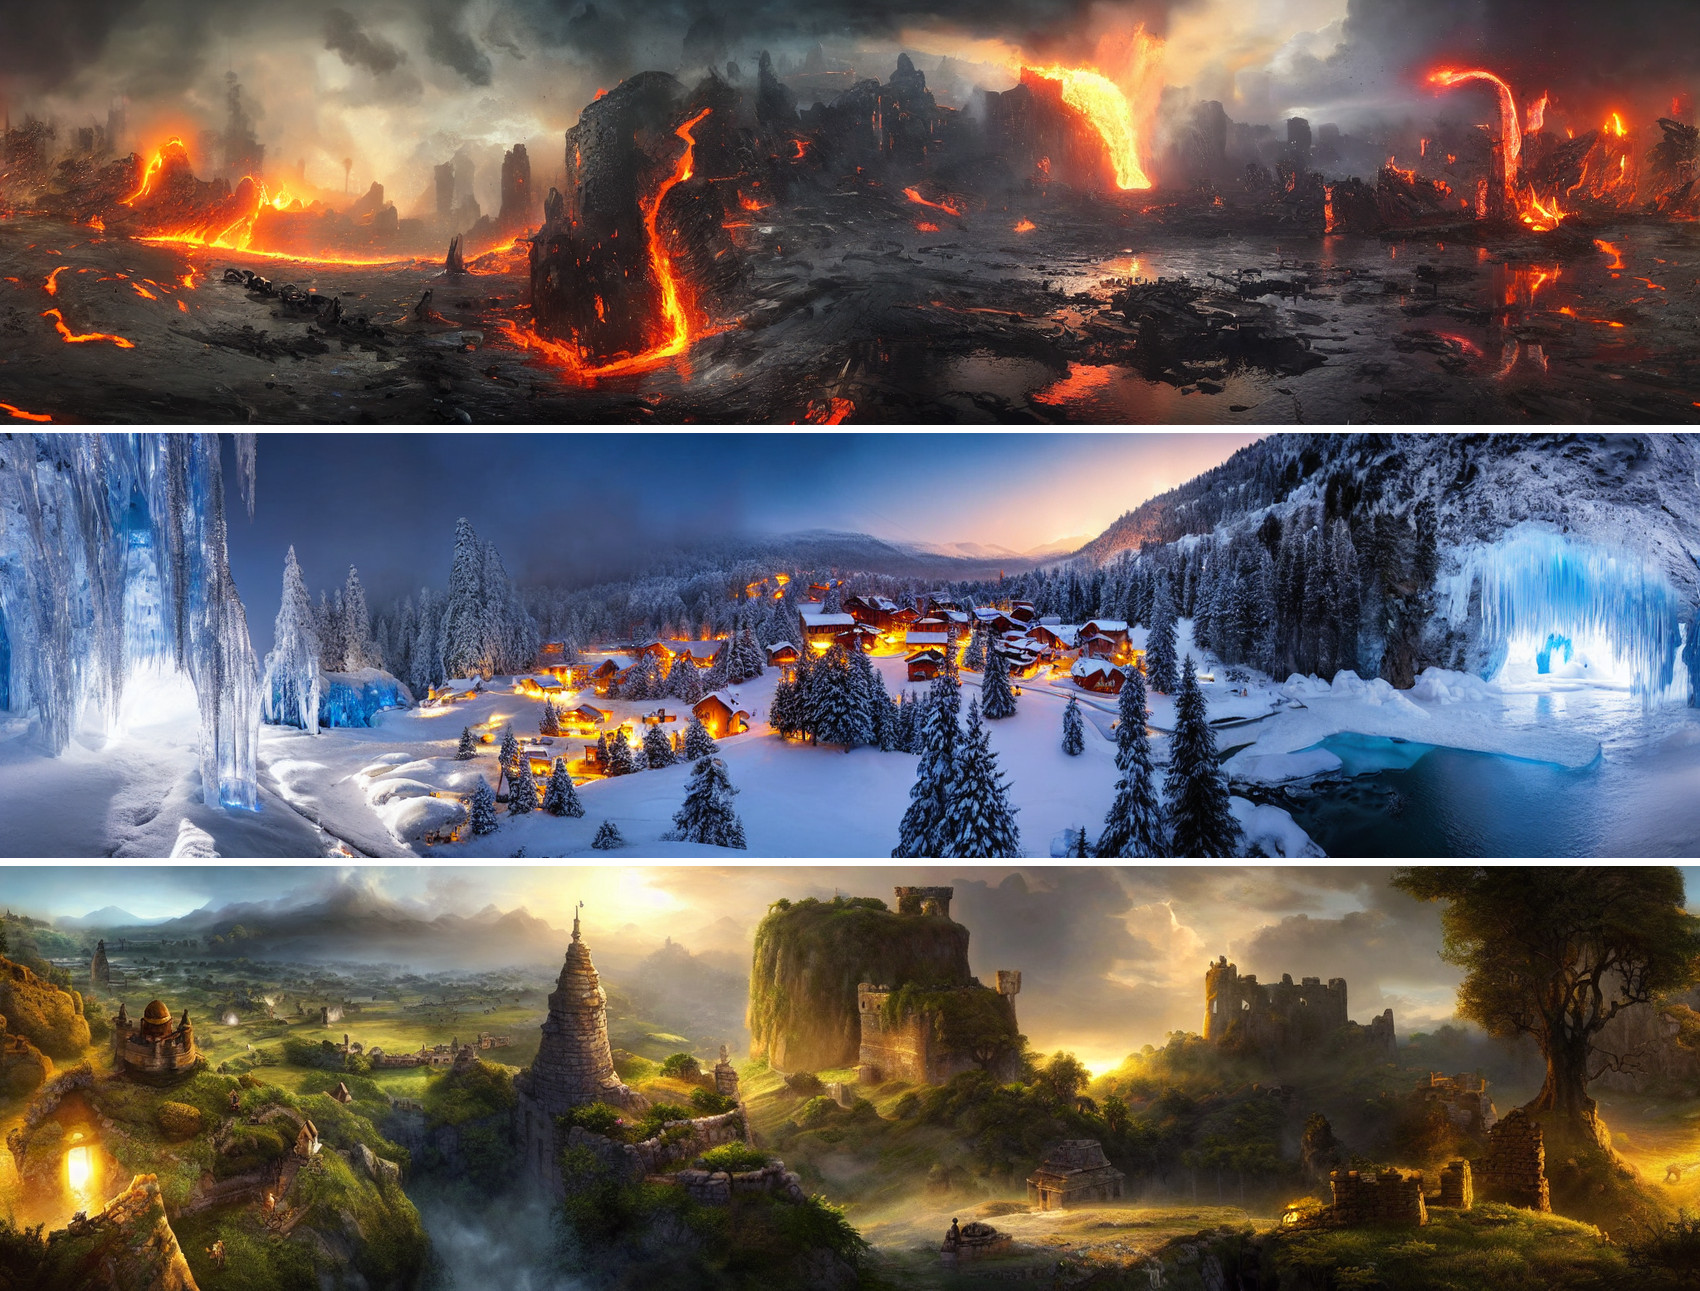
\includegraphics[width=0.66\textwidth]{fig/hero.jpg}\par
\vspace{-5pt}
\vspace{1pt}
\captionof{figure}{Three finished worlds, each $2048\times512$\,px from the submitted notebook and \emph{nothing but} Stable Diffusion v1.5 --- no source images, no fine-tuning. Top to bottom: \thm{volcanic\_lava\_world\,+\,flooded\_metropolis} (seed 201), \thm{arctic\_ice\_cave\,+\,cozy\_village\_snowfall} (seed 1002, region-conditioned), \thm{fantasy\,+\,medieval} (seed 1001). In each, the left and right edges are the \emph{same} edge --- cylinders, not strips (Table~\ref{tab:seam}).}
\label{fig:hero}
\vspace{7pt}
}]

\section{Goal and concept}

One run of my notebook produces a wide panorama of an imagined world whose
\textbf{left and right edges join perfectly}. Roll the image sideways by any
amount, wrap it around a cylinder or use it as a 360$^\circ$ backdrop, and no seam
appears anywhere. The user picks \textbf{one or two} themes from a 50-entry menu I
wrote (plus a \tw{custom} slot); with two themes the notebook builds a
\emph{single} world that fuses them --- lava rivers running through a drowned
city, neon towers encrusted in coral, an ice cave that opens onto a lantern-lit
village and closes back into ice as you travel around the loop.

This is harder than it sounds. SD v1.5 was trained at $512\times512$; asked
directly for $2048\times512$ it paints roughly four $512$-ish scenes glued
together, with duplicated skylines and warped geometry, because nothing in its
training distribution has that shape --- and nothing in the model makes the left
edge agree with the right edge, so a panorama generated normally is a
\emph{strip} with an obvious join.

On top of the course rules I set two constraints: \textbf{inference time only} (no
fine-tuning, no LoRA) and \textbf{zero source images} --- 0 of the 10 permitted.
Every submitted pixel comes from the stock SD v1.5 weights; the contribution is
the sampling schedule around them, written out in the notebook rather than
imported from a library.

\section{Method}

\subsection{MultiDiffusion, re-implemented}

The backbone is MultiDiffusion~\cite{multidiffusion}. A single shared latent
canvas $x_t$ of size $\tfrac{W}{8}\times\tfrac{H}{8}$ is kept. At every denoising
step the canvas is cut into overlapping $64\times64$-latent windows
($=512\times512$\,px, exactly SD v1.5's native shape); one ordinary DDIM step
$\Phi$ runs on each window independently; the results are averaged back:
\begin{equation}
x_{t-1}=\Big(\textstyle\sum_i \mathcal{S}_i^{\!\top}\,\Phi\big(\mathcal{S}_i x_t\big)\Big)
\oslash\Big(\textstyle\sum_i \mathcal{S}_i^{\!\top}\mathbf{1}\Big),
\end{equation}
where $\mathcal{S}_i$ crops window $i$ and $\oslash$ is elementwise division, so
every latent cell becomes the average of every window opinion that covered it.
Each window is a problem the UNet was trained to solve; the averaging is what
forces neighbours to agree on one scene over the 50 steps. No weight is touched
and no tensor exceeds $64\times64$ latents, which is why $2048\times512$ fits on a
free T4.

\subsection{Extension 1: circular windows}

The published method tiles a strip. I make the window list \emph{wrap}: columns
run $\{0,s,2s,\dots\}$ across the full latent width and each window indexes its
columns modulo that width (\tw{arange(w0,w1) \% W}), so a window starting near the
right edge continues onto the left edge. Both ends therefore share windows from
step~1 and are denoised as one continuous surface: \textbf{nothing is stitched
afterwards}, the loop is a property of the sampling. That fixes the latents; the
VAE decoder has a receptive field of its own, so before decoding I wrap 8 latent
columns around each side and crop the corresponding 64\,px off afterwards.

\subsection{Extension 2: multi-branch theme conditioning}

The obvious way to combine two themes is to concatenate them into one prompt. I
measured what that costs: CLIP's text encoder has a hard \textbf{77-token} context
and silently discards the rest, and a fused two-theme prompt
(\thm{cyberpunk\,+\,medieval}) measures \textbf{97 tokens} --- so \textbf{20 tokens
are dropped without warning}, and what gets cut is the tail, i.e.\ the quality
suffix, every time.

So I never concatenate. My sampler accepts $K$ conditioning \emph{branches}, each
with its own embedding \emph{per window}, plus a weight matrix; one UNet call
carries the unconditional pass and all $K$ branches, whose classifier-free
guidance~\cite{cfg} directions are added:
\begin{equation}
\hat\epsilon=\epsilon_u+g\sum_{k=1}^{K}w_k\big(\epsilon_k-\epsilon_u\big),\qquad \textstyle\sum_k w_k=1 .
\end{equation}
Four strategies fall out, differing \emph{only} inside \tw{build\_conditioning} ---
everything downstream is shared, which is what makes Fig.~\ref{fig:fusion} a fair
comparison. \tw{compose} (default) sets $K{=}2$ so both prompts act on every
pixel, combined in noise space as in composable diffusion~\cite{composable};
neither prompt is ever truncated because neither is ever concatenated.
\tw{regions} keeps $K{=}1$ but gives every window its own interpolated embedding
along a circular raised-cosine field
$w(u)=\mathrm{clip}\big[\big(\tfrac{1}{2}(1{+}\cos 2\pi u)-\tfrac12\big)\sigma+\tfrac12\big]$,
so each theme owns one side of the loop with two blended hand-off bands.
\tw{blend} uses one averaged embedding everywhere, and \tw{single\_prompt} is the
naive concatenation, kept as a control.

\subsection{Fitting a free T4}

MultiDiffusion calls \tw{scheduler.step()} once per window per timestep, out of
order, so the scheduler must be stateless: DDIM~\cite{ddim} is, SD v1.5's default
PNDM is not --- it would silently corrupt its own history --- and the notebook
swaps it and asserts the swap. The UNet runs in fp16 but the fusion accumulator is
fp32, because averaging up to eight overlapping fp16 predictions per cell is
exactly where rounding shows up as banding. Windows are batched (halved
automatically when two branches are active, to keep the real UNet batch constant),
the stride is exposed (16 rather than the reference's hard-coded 8, halving the
work), and VAE decoding falls back to tiled decoding on OOM. Initial noise is
drawn on the \textbf{CPU} generator, whose RNG is identical across GPUs, so a seed
reproduces the same image on any machine (\S\ref{sec:repro}). The safety checker
is not loaded: it generates nothing, costs ${\sim}1.2$\,GB and returns black
images on false positives, a real risk for stylised landscape art.

\section{Data and resources}

\textbf{Source or training images: none} --- zero of the ten permitted. There is no
image input, no upload step and no \tw{data.zip}, and nothing was fine-tuned. The
50-theme menu, the quality suffix and the negative prompt are my own text;
Table~\ref{tab:weights} lists every pretrained weight the notebook loads and where
it comes from. Software: \tw{diffusers} (a weight loader and \tw{DDIMScheduler}
only --- the sampler is written out in the notebook), \tw{transformers},
\tw{torch}, \tw{numpy}, \tw{PIL}. All compositing and labelling happens inside the
notebook with PIL; no image is edited in an external tool and no text label is
ever asked of the model.

\begin{table}[t]
\centering\small
\caption{Every pretrained weight loaded by the notebook.}
\label{tab:weights}
\begin{tabularx}{\columnwidth}{@{}>{\raggedright\arraybackslash}p{1.95cm}@{\hspace{4pt}}>{\raggedright\arraybackslash}X@{}}
\toprule
\textbf{Weight} & \textbf{Role and source}\\
\midrule
SD v1.5\newline(fp16) &
\textbf{Generates every submitted pixel.} \tw{stable-diffusion-v1-5/} \tw{stable-diffusion-v1-5} on Hugging Face,\newline
\url{https://huggingface.co/stable-diffusion-v1-5/stable-diffusion-v1-5}, loaded with \tw{from\_pretrained}. Ships its own CLIP ViT-L/14 \emph{text} encoder, the VAE and the scheduler config.\\
\addlinespace[2pt]
CLIP ViT-L/14 &
\textbf{Scores finished images only; generates nothing.} \tw{openai/clip-vit-large-patch14},\newline
\url{https://huggingface.co/openai/clip-vit-large-patch14}. Used in Step~9 to rank candidates --- the ``pretrained reward model'' carve-out. Setting \tw{USE\_CLIP\_RANKING=False} disables it and the notebook still runs.\\
\addlinespace[2pt]
\emph{(not loaded)} & The SD safety checker is explicitly disabled. No SDXL/FLUX, no third-party SD v1.5 checkpoint, LoRA or DreamBooth model exists anywhere in the notebook.\\
\bottomrule
\end{tabularx}
\end{table}

\section{Experimental setup}

\begin{table}[t]
\centering\small
\caption{Settings for the submitted panoramas.}
\label{tab:setup}
\begin{tabularx}{\columnwidth}{@{}>{\raggedright\arraybackslash}p{1.85cm}@{\hspace{4pt}}>{\raggedright\arraybackslash}X@{}}
\toprule
Canvas & $2048\times512$ (also $1536\times768$), multiples of 64\\
Window / stride & $64\times64$ latents ($512$\,px) / 16 cells $\Rightarrow$ 16 windows per step, every cell covered ${\geq}4\times$\\
Sampler & DDIM, 50 steps, CFG 7.5; \tw{compose} ($K{=}2$, $\lambda{=}0.5$) or \tw{regions} (sharpness 2.0)\\
Runtime & fp16 UNet/VAE with an fp32 fusion accumulator; 4 windows per UNet call (2 when $K{=}2$); seeds \tw{BASE\_SEED}$+i$ drawn on the CPU generator; $\pm 8$ latent columns of circular padding before decoding, then cropped\\
Prompt & \tw{"\{theme\}, seamless wide panorama, sweeping vista, single horizon, highly detailed, atmospheric, cinematic lighting, digital matte painting"} (${\leq}55$ tokens)\\
Negative & seam, stitching artifact, repeating/tiling pattern, duplicate objects, split screen, multiple horizons, repeated skyline, text, watermark, border (66 tok.)\\
\bottomrule
\end{tabularx}
\end{table}

Table~\ref{tab:setup} gives the settings. Each run renders
\tw{NUM\_CANDIDATES} seeds, saves every candidate at full resolution, and writes a
JSON log with the checkpoint id, scheduler config, resolved prompts, canvas,
steps, guidance, window/stride, every seed and the measured scores, so any image
can be regenerated exactly. Selection is quantitative: CLIP ViT-L/14~\cite{clip}
scores six square crops taken \emph{around the loop} (a panorama is four times
wider than CLIP's square input), a theme's score is its best crop, and the
candidate's score is the \emph{worst} of the two theme scores --- penalising a
candidate that quietly dropped a theme. Anything above a seam ratio of 4.0 is
disqualified.

\begin{figure*}[t]
\centering
\newcommand{\ctrl}[2]{\begin{subfigure}{0.325\textwidth}\includegraphics[width=\linewidth]{#1}\caption{#2}\end{subfigure}}
\ctrl{fig/circ_off_c.jpg}{circular windows \textbf{off} --- seam 6.39}\hfill
\ctrl{fig/circ_on_c.jpg}{circular windows \textbf{on} --- seam 0.97}\hfill
\ctrl{fig/fus_0_c.jpg}{\tw{single\_prompt}: a dry city, no reef}\\[3pt]
\ctrl{fig/fus_1_c.jpg}{\tw{blend}: a washed-out midpoint}\hfill
\ctrl{fig/fus_2_c.jpg}{\tw{regions}: reef centre, towers at both ends}\hfill
\ctrl{fig/fus_3_c.jpg}{\tw{compose}: a submerged neon city}
\caption{\textbf{Controls, all from one seed} (\thm{cyberpunk\,+\,underwater},
$1024\times512$, 30 steps, identical in every other respect). \textbf{(a--b)} the
circular ablation, both rolled by 50\% so the join sits in the centre: without
wrapping, two unrelated scenes are butted together mid-frame; with it, one
continuous world. \textbf{(c--f)} the four fusion modes --- the naive concatenation
(c) drops the underwater theme outright and paints a night skyline above water,
as the 77-token measurement predicts, while only \tw{compose} (f) puts both
themes in every pixel.}
\label{fig:fusion}
\end{figure*}

\section{Results and analysis}

\subsection{Does it actually loop?}

The claim needs a number, not an impression. I define the \textbf{seam ratio} as
the mean absolute difference between the first and last image columns divided by
the mean absolute difference between \emph{neighbouring} columns:
\begin{equation}
R=\overline{|I_{:,0}-I_{:,W-1}|}\;\big/\;\overline{|I_{:,j+1}-I_{:,j}|}.
\end{equation}
$R\approx1$ means the wrap-around join is statistically indistinguishable from any
other pair of adjacent columns --- there is no special column --- whereas a strip
merely cropped to size blows up. Across \textbf{28 panoramas in 12 configurations}
the measured value averages $\mathbf{1.12}$ (median 1.13, s.d.\ 0.23, worst case
1.62; 26 of 28 below 1.5), Table~\ref{tab:seam}.

\begin{table}[t]
\centering\scriptsize
\caption{Every submitted configuration and the seam ratio measured on each
finished panorama ($\approx 1$ = a perfect loop). All $2048\times512$ except
$^\dagger$ ($1536\times768$). Mean over all 28: \textbf{1.12}.}
\label{tab:seam}
\setlength{\tabcolsep}{2.5pt}
\begin{tabular}{@{}lr@{\hspace{7pt}}lr@{}}
\toprule
\textbf{Theme(s)} & \textbf{Seam} & \textbf{Theme(s)} & \textbf{Seam}\\
\midrule
\thm{cyberpunk} & 1.16 & \thm{alien\_jungle\,+} & 1.29\\
 & 1.27 & \quad\thm{desert\_planet} & 1.36\\
 & 0.87 & \thm{abandoned\_park\,+} & 1.11\\
\thm{stained\_glass}$^\dagger$ & 1.11 & \quad\thm{toy\_world}$^\dagger$ & 1.24\\
 & 1.14 & \thm{ink\_wash\_mtns\,+} & 1.53\\
\thm{cyberpunk\,+} & 1.23 & \quad\thm{dragon\_spire} & 1.27\\
\quad\thm{underwater} & 1.34 & \thm{volcanic\_lava\,+} & 1.20\\
 & 0.96 & \quad\thm{flooded\_city} & 0.88\\
\thm{arctic\_ice\_cave\,+} & 0.76 & \thm{giant\_tree\,+} & 1.00\\
\quad\thm{cozy\_village} & 1.47 & \quad\thm{biopunk\_city} & 1.08\\
 & 0.89 & \quad(2 separate runs) & 0.91\\
\thm{fantasy\,+} & 1.62 & & 1.12\\
\quad\thm{medieval} & 1.19 & \thm{gothic\_courtyard\,+} & 0.92\\
 & 0.79 & \quad\thm{abandoned\_park} & 0.61\\
\bottomrule
\end{tabular}
\end{table}


\subsection{Control 1: is the circular machinery doing anything?}

The honest test is the same theme, seed and steps with window wrapping switched
off; the notebook runs this pair automatically. Over \textbf{12 paired runs} the
seam ratio is \textbf{7.94} on average with wrapping \emph{off} (range
5.01--14.63) versus \textbf{1.05} with it \emph{on} (0.72--1.36): a mean
$\mathbf{7.6\times}$ improvement on identical inputs, never below $5.4\times$.
Fig.~\ref{fig:fusion}(a--b) is a representative pair: without the wrap the two
ends are visibly different scenes butted together, with it the join is
unfindable; the largest gap measured was $14.63\to1.36$.

\subsection{Control 2: what the four fusion modes do}

Fig.~\ref{fig:fusion}(c--f) renders all four strategies from one seed, and the
differences are systematic rather than cosmetic. \tw{single\_prompt} \emph{loses
the second theme entirely} --- it paints a dry neon skyline reflected in water,
with nothing submerged, exactly as the token measurement predicts. \tw{blend}
washes out into a midpoint that is neither city nor reef, because the average of
two distant CLIP embeddings is rarely either concept. \tw{regions} gives each
theme its own territory: reef through the centre, city towers at both ends of the
loop. \tw{compose} spreads both themes over every pixel and was the only mode to
produce genuinely hybrid architecture: coral-encrusted skyscrapers lit by their
own neon. The cost matches
the theory --- $K{+}1$ passes per window instead of two --- and over nine paired
control runs \tw{compose} took $\mathbf{1.53\times}$ the single-branch modes
(1.50--1.63$\times$), which were within a second of each other.

\subsection{Control 3: is the re-implementation correct?}

\tw{diffusers} ships its own (now deprecated) MultiDiffusion sampler,
\tw{StableDiffusionPanoramaPipeline}. Since mine is written from scratch, the
notebook runs the reference on the same checkpoint, canvas, seed and step count as
an independent check: over 12 pairs the seam ratios are statistically
indistinguishable (reference $0.95\pm0.22$ versus mine $0.99\pm0.22$), i.e.\ the
re-implementation behaves like the published method.

It also surfaced a real limitation of the reference: with
\tw{circular\_padding=True} it scatters each finished window back using
\emph{canvas} row indices rather than window-local ones, so any canvas taller than
one window raises a shape mismatch (and the pipeline is unmaintained past
\tw{diffusers}~0.33.1). Mine never addresses a window by canvas coordinates,
which is why the $768$-tall panoramas here work; the cross-check is pinned to
512\,px for that reason.

\subsection{Reproducibility}
\label{sec:repro}

Two independent Colab sessions on different days, with the same seeds and
settings, produced \textbf{byte-identical PNGs} (MD5 \tw{f737a887\dots},
\tw{16f0c451\dots}, \tw{8a6e4445\dots}, seeds 1000--1002 of the \thm{cyberpunk}
run) --- the practical payoff of the CPU noise generator: re-running the notebook
returns \emph{these} images, not merely similar ones.

\subsection{What I learned, and what does not work}

\textbf{Tokenisation, not attention, is what kills fused prompts.} I expected
\tw{single\_prompt} to blur the two themes; instead it deletes one, and the token
count says why --- measuring the prompt beat staring at the image. Relatedly,
\textbf{averaging is what buys global coherence}, at the price of slightly softer
local contrast where windows pile up --- which is why stride 16 ($4\times$
coverage) looked no worse to me than the reference's stride 8 ($8\times$) while
costing half as much.

\textbf{Limitations.} Composition is seed-sensitive --- SD v1.5's model card flags
multi-object compositionality as a weak point, and with distant concepts some
seeds land on a genuine hybrid and others on a compromise that reads as neither,
hence several seeds per run and a worst-of-both-themes ranking. High-contrast
pairs (\thm{volcanic\_lava\,+\,arctic\_ice\_cave}) tend to cancel under \tw{compose}
and are better served by \tw{regions}. The seam metric certifies the wrap, not
semantic continuity: a world can loop perfectly and still change mood across the
frame. Object-level fidelity stays SD v1.5's --- small figures and animals in the
busier worlds are often malformed under magnification, and no sampling schedule
fixes that.

\subsection{Rule compliance}

SD v1.5 (Table~\ref{tab:weights}) generated every submitted pixel --- no other
generative model, no fine-tuning, no source images (hence no \tw{data.zip}), CLIP
confined to scoring. The deliverable is one \tw{.ipynb} that runs end to
end on a Colab T4 with all cell outputs saved, and every visual is a static PNG.

\begin{thebibliography}{9}\footnotesize
\setlength{\itemsep}{1pt}
\bibitem{multidiffusion} O.~Bar-Tal, L.~Yariv, Y.~Lipman, T.~Dekel.
\emph{MultiDiffusion: Fusing Diffusion Paths for Controlled Image Generation.} ICML 2023. arXiv:2302.08113.
\bibitem{composable} N.~Liu, S.~Li, Y.~Du, A.~Torralba, J.~B.~Tenenbaum.
\emph{Compositional Visual Generation with Composable Diffusion Models.} ECCV 2022. arXiv:2206.01714.
\bibitem{ldm} R.~Rombach, A.~Blattmann, D.~Lorenz, P.~Esser, B.~Ommer.
\emph{High-Resolution Image Synthesis with Latent Diffusion Models.} CVPR 2022. arXiv:2112.10752.
\bibitem{ddim} J.~Song, C.~Meng, S.~Ermon. \emph{Denoising Diffusion Implicit Models.} ICLR 2021. arXiv:2010.02502.
\bibitem{cfg} J.~Ho, T.~Salimans. \emph{Classifier-Free Diffusion Guidance.} NeurIPS 2021 Workshop. arXiv:2207.12598.
\bibitem{clip} A.~Radford et al. \emph{Learning Transferable Visual Models From Natural Language Supervision.} ICML 2021. arXiv:2103.00020.
\bibitem{diffusers} P.~von Platen et al. \emph{Diffusers: State-of-the-art diffusion models.} \url{https://github.com/huggingface/diffusers}.
\end{thebibliography}

\end{document}
